
%************************************************
\chapter{Evolución de codificadores JPEG}\label{ch:resultados_evolucion}
%************************************************

% ============================================================
\section{Introducción al Cómputo Evolutivo}
% ============================================================

El \gls{Cómputo Evolutivo} es una rama de la Inteligencia Artificial que se define
por los tipos de algoritmos en los que se enfoca. Son algoritmos que utilizan
el concepto de evolución y selección natural para resolver problemas de cómputo. Son
problemas de optimización en el sentido matemático. Es decir, se concentran en
encontrar un máximo local o un mínimo local utilizando heurísticas.

% ============================================================
\section{Algoritmos Evolutivos}
% ============================================================

Las características que los Algoritmos Evolutivos tienen en común son:

\begin{itemize}
   \item Definen una población.
   \item Definen un método de selección.
   \item Utilizan mutación y recombinación junto con el método de selección para
      mejorar la población a lo largo de varias generaciones.
\end{itemize}

Aunque comparten la misma idea, se definen distintos tipos de algoritmos con
respecto a la manera en que concretizan estas características.

\begin{itemize}
   \item La \emph{Programación Genética} \cite{GenProg} tiene conjuntos de
      programas como su población. Su función de aptitud es la capacidad de un
      programa para resolver cierto problema. Los programas se representan como
      árboles de sintaxis, y de esta manera se define la mutación y recombinación como
      operaciones en árboles.
   \item La \emph{Programación Evolutiva} es similar a la Programación Genética
      pero lo que evoluciona son los parámetros de los programas, no su
      estructura. Usualmente se utilizan para evolucionar máquinas de
      predicción. Las poblaciones consisten de máquinas de estado finito. El
      método de selección consiste de evaluar la función delta de cada miembro
      de la población para un conjunto de entradas de entrenamiento. Para cada
      elemento de una entrada, se compara la evaluación de la función delta con
      el valor de la siguiente entrada. Los miembros de la población más aptos son
      los que producen mejores predicciones.
   \item Los \emph{Algoritmos Genéticos} definen sus soluciones con
      representaciones genéticas. En una representación genética, una solución,
      el fenotipo, es representada por una arreglo de valores, su genotipo.
      Usualmente estas representaciones son arreglos de bits, pero pueden ser
      arreglos de cualquier tipo. Ya que la representación de cada miembro es
      un arreglo, las operaciones de recombinación y mutación son simples de
      implementar.
\end{itemize}

El algoritmo que se presenta en la sección \ref{sec:GA} es un algoritmo
genético. La población consiste de codificadores JPEG, que son representados
genéticamente por sus respectivas tablas de cuantificación.

Al comienzo de la sección se describió la estructura común de un algoritmo
evolutivo. A continuación se definen de una manera general, con un enfoque hacia
los algoritmos genéticos.

Un algoritmo evolutivo itera sobre una población, produciendo nuevas
generaciones hasta que se cumpla un criterio de terminación.

\subsection { Inicialización de la Población }

La manera en que se inicializa la población depende del conocimiento que se tiene
\emph{a priori} sobre el espacio de búsqueda. Si el espacio es grande y no se
conocen las características de buenas soluciones, cada miembro se inicializa al
azar. En el caso de la evolución genética, esto significa un arreglo de valores
aleatorios. Si se cuenta con información que puede ser de ayuda, inicializar la
población al azar probablemente no es la mejor idea. De ser posible, es bueno
escoger una población inicial cuyos miembros tengan una mayor probabilidad de
estar cerca de mínimos o máximos locales distintos. Tener a \emph{toda} la
población cerca de un mínimo o máximo puede ser contraproducente, ya que es posible que el
proceso evolutivo no encuentre mejores soluciones. Le llamamos cromosoma a la
representación genética de un elemento de la población.

\subsection { Función de aptitud }

Existe una función que recibe un miembro de la población y regresa un valor
numérico.  No es un requerimiento que la función de aptitud regrese un número,
basta con que el dominio de la función tenga un orden parcial. El propósito del
cada iteración del algoritmo evolutivo es encontrar nuevos miembros del espacio
de búsqueda con el propósito de minimizar o maximizar la función de aptitud. En
cuestión de desempeño, la función de aptitud es donde un algoritmo evolutivo va
a pasar la mayor parte de su tiempo.

Al principio de cada iteración, se evalúa la aptitud de cada miembro de la población.

\subsection { Método de selección }

Cada iteración reemplaza la generación actual con una nueva. Esto se hace
tomando elementos de la vieja generación y generando nuevos elementos
utilizando operadores evolutivos.

Hay distintas maneras en las que se escogen los \emph{supervivientes} de cada
generación.

El método más simple es el \emph{Método Elitista}, en el que siempre se escogen
los elementos más aptos. Como menciona Koza \cite{koza} en la introducción de su
libro de programación genética, este método tiene la desventaja de que
disminuye la diversidad. Por ejemplo, es posible que para alguna generación,
exista algún elemento en particular que no tenga alta aptitud, pero pueda
convertirse en una nueva y mejor solución con una mutación simple. El método
Elitista no le da oportunidad a este tipo de elementos.

El \emph{Método de Ruleta} hace que la probabilidad de seleccionar un elemento en
particular sea proporcional a su aptitud. Si $f$ es la función de aptitud y la
población es de $N$ elementos, entonces para un elemento $e_i$, su probabilidad
de ser seleccionado es $P(e_i) = f(e_i) / \sum_{k=0}^{N} f(e_k)$.

El \emph{Método de Rango} (traducido del Inglés \emph{rank selection}) es similar al
de la Ruleta, pero en lugar de que la probabilidad sea proporcional a la
aptitud, es proporcional al \emph{orden}. La población se ordena de menor
aptitud a mayor aptitud. La probabilidad para que cada elemento sea
seleccionado crece linealmente.

\subsection { Operadores evolutivos }

Hay dos maneras en las que se generan nuevos miembros para la nueva generación:

\begin{itemize}
      \item Recombinación
      \item Mutación
\end{itemize}

La recombinación toma dos padres y a partir de ellos genera uno o más nuevos
elementos. Para una representación genética, Koza \cite{koza} recomienda
escoger un \emph{Punto de Cruza} (un índice dentro del cromosoma) y generar dos
hijos. Un hijo tiene la primera parte del primer padre y la segunda parte del
segundo padre. El segundo hijo tiene la segunda parte del primer padre y la
primera parte del segundo padre.

La mutación consiste de seleccionar un padre y efectuar un cambio al azar. Para
algoritmos genéticos, esto normalmente significa escoger algún elemento del
cromosoma y cambiarlo. Si la codificación es binaria, basta con cambiar un 1 a
un 0 o viceversa.

La recombinación ayuda a encontrar elementos más aptos con la esperanza de que
al recombinar, el nuevo elemento tenga lo mejor de ambos padres. La mutación
agrega diversidad, aumentando la probabilidad de que el proceso evolutivo
encuentre nuevas y mejores soluciones fuera de un mínimo o máximo local.

\subsection { Criterio de terminación }

El algoritmo necesita terminar. Puede elegirse un número máximo de generaciones
para evitar que corra indefinidamente. Se puede elegir un umbral de aptitud tal
que una solución que lo cruce pueda sea considerada suficientemente buena.
También puede medirse la velocidad a la que cambia la aptitud generación tras
generación. Se puede escoger un umbral tal que si los elementos más aptos de
dos o más generaciones sucesivas tienen una diferencia entre sus aptitudes
dentro del umbral, el algoritmo decida que ha convergido y termine.

% ============================================================
\section{Método para la evolución de codificadores JPEG} \label{sec:GA}
% ============================================================

\subsection{Población}

El espacio de búsqueda consiste de tablas de cuantificación de $8\times8$. Cada
coeficiente de una tabla válida es un número positivo de 8 bits. El tamaño del
espacio de búsqueda es entonces $256^{64}$.

El tamaño de la población que se eligió es de 48 tablas de cuantificación. Se
eligió este número para mantener el desempeño del algoritmo en un nivel
aceptable.

La tabla que tiene todos sus coeficientes iguales a 1, denominada
\emph{\gls{tabla unitaria}}, tiene dos propiedades que nos interesan. Primero,
la tabla unitaria es la que obtiene la mejor calidad posible en las imágenes
resultantes, ya que minimiza la pérdida de información. La segunda propiedad es
que la tabla unitaria produce la imagen más grande posible con JPEG
\emph{baseline}. Como la tabla unitaria presenta los dos extremos de calidad y
tamaño, se incluye en la población inicial.

El resto del conjunto se llena de tablas con valores aleatorios entre 1 y 25.
Este límite se eligió al observar las tablas obtenidas al correr el algoritmo
con una población inicial aleatoria y observar que las tablas raramente tienen
coeficientes mayores a 30. Acotar los posibles valores de cada coeficiente
ayuda a encontrar mejores soluciones en menos tiempo.

Antes de iniciar la evolución, se comprime la imagen con la tabla unitaria,
dando un punto de referencia para la calidad óptima y para el máximo tamaño.
Esto es necesario para la función de aptitud \ref{eq:fitness}.

\subsection{ Selección }

Para el método de selección, se usa una distribución de probabilidad de Pareto,
que es un tipo de Ley Potencial.

La función general para la distribución de probabilidad de Pareto es $\frac{
\alpha x_m^{\alpha} } { x^{\alpha + 1} }$ donde $x_m$ es el valor mínimo y
$\alpha$ es un entero positivo. Mientras $\alpha$ crece, es más alta la
probabilidad del valor mínimo.

Con un valor mínimo de 1 y $\alpha=1$, la función de distribución acumulativa
es $F(x) = 1 - (1/x)$ con $x$ un entero positivo. Si generamos un entero
positivo $x$ con una función pseudo-aleatoria uniforme, $F(x)$ resulta en un
número aleatorio en la distribución de probabilidad de Pareto en $[0, 1]$.

La población se ordena según aptitud en orden descendente. Para seleccionar un
elemento, se toma un valor aleatorio de Pareto $P$, y obtenemos $i = \lfloor P*N
- 1 \rfloor$, donde $N$ es el tamaño de la población, $i \in [0, N-1]$ es el índice del
arreglo para el elemento seleccionado.

Con una distribución de probabilidad de Pareto, es altamente probable que el elemento seleccionado esté al inicio del arreglo, pero siempre existe una probabilidad de escoger cualquier elemento de la población.

\subsection { Función de aptitud }

La calidad de la compresión se determina haciendo una decodificación y
comparando la imagen resultante con la original pixel por pixel. Las
diferencias absolutas se suman. No se utiliza MSE (Error cuadrático medio) por
la enorme cantidad de pixeles y la sensibilidad del algoritmo a errores de
precisión. En lugar de implementar un decodificador JPEG, se incluye un paso de
decodificación en la función principal de procesamiento de bloques. Los
detalles de este proceso se explican en el capítulo \ref{ch:implementacion}.

El tamaño es más fácil de comparar que la calidad de la imagen. Tan solo es
necesario ver cuántos bits pesa la imagen resultante comparada con el tamaño
máximo, obtenido con la tabla unitaria.

Se tienen dos garantías. Cualquier tabla de cuantificación comparada con la
unitaria va a resultar en mayor compresión y en menor calidad, siempre y cuando
la tabla a comparar no sea en sí una tabla unitaria.

Sea $T$ una tabla de la población y sea $T_0$ la tabla unitaria.

Definimos la función de aptitud como:

\begin{equation}
f(T) = \frac{e(T)}{e(T_0)} + \alpha \Big(\frac{s(T)}{s(T_0)}\Big)
\end{equation}\label{eq:fitness}

donde $e(T)$ es el error de compresión y $s(T)$ es el tamaño de la
imagen. $\alpha$ es una constante que se usa para ajustar la importancia que se le
da al tamaño sobre la compresión o vice versa.

Es importante notar que los dos términos se afectan mutuamente. Una tabla que tiene mayor
compresión va a tener un mayor error, y una tabla con menor compresión resulta
en una imagen de mayor calidad. En otras palabras, cuando el primer término
disminuye, el segundo crece. Cuando el segundo término crece, el primero
disminuye.

La meta es encontrar $T$ tal que $f(T)$ es mínima. La relación entre los
dos términos permite que el algoritmo converja.

El valor de $\alpha$ controla el proceso de minimización. Mientras mayor sea
$\alpha$, más peso de aptitud tiene el tamaño de la imagen.

Habiendo probado varios valores distintos, se encontró que un valor de $\alpha
= 10$ resulta en imágenes que son indistinguibles de las originales, con un alto
nivel de compresión.

\subsection {Mutación y Recombinación}

En cada iteración, se genera una nueva población basada en la anterior.

Cada nuevo elemento tiene una probabilidad de 70\% de ser obtenido por mutación
de un elemento de la generación anterior, un 25\% de ser el resultado de
recombinación de dos elementos, y un 5\% de ser una copia directa de un
elemento de la generación anterior. Todos los elementos de la generación
anterior se escogen con el método de selección descrito anteriormente.

El método de dar un 5\% de probabilidad de obtener una copia directa se hace
siguiendo la descripción de Koza de algoritmos evolutivos. En lugar de mantener
la mejor solución a lo largo de la evolución, se deja que el algoritmo intente
mantenerla en la población. La elección de probabilidades de 70\% y 25\% entre
mutación y recombinación se hizo heurísticamente. Para este problema no se
encontraron buenos resultados usando la recombinación como principal
herramienta para obtener nuevas soluciones. Sin embargo, una probabilidad de
recombinación de 25\% resulta en poblaciones con aptitud más minimizada,
comparando con el caso en el que no se realiza recombinación.

El proceso de mutación es como sigue: Se escoge un coeficiente de la tabla y se
le suma un valor en $[-4, 4]$ con probabilidad uniforme. Si el coeficiente es
negativo como resultado de la mutación, se corrige a 1, porque JPEG asume que
las tablas consisten de enteros positivos. Se hace lo mismo para valores
grandes. Si el coeficiente resulta mayor a 255, se corrige a 255.

El proceso de recombinación ocurre primero seleccionando dos tablas. El método
de selección incluye un mecanismo para evitar seleccionar la misma tabla dos
veces. Teniéndose los dos padres, Padre A y Padre B, La tabla hijo es el
resultado de, para cada coeficiente, escoger el valor correspondiente del Padre
A o del Padre B, con un $50\%$ de probabilidad de venir de cualquiera de ellos.

Se intentó el método de punto de cruza descrito por Koza, pero el método
descrito aquí resultó ser más efectivo para este problema.

\subsection { Criterio de terminación }

El algoritmo decide terminar cuando sucede alguno de los siguientes casos:

\begin{itemize}
\item El número de generaciones llega a 500
\item Dado el individuo más apto de generación previa $x_p$ y el de la generación actual, $x_0$, sucede cuatro veces consecutivas que $f(x_p) - f(x_0) \leq 0.0001$, donde $f$ es la función de aptitud \ref{eq:fitness}.
\end{itemize}

Al final de la evolución, se toma la tabla ganadora y se usa como entrada para
el codificador \gls{JPEG}.

\section{Codificador Evolutivo}

El nombre del proyecto final es \emph{gp\_encoder}. Consta de un algoritmo
evolutivo que utiliza a DummyJPEG para su función de aptitud y a TinyJPEG
para codificar la imagen resultante.

% ============================================================
\section{Conjuntos de prueba} \label{sec:testset}
% ============================================================

El proyecto está dividido en tres partes: TinyJPEG: la implementación de JPEG
con compresión \emph{baseline} basada en la especificación \cite{jpeg-spec};
DummyJPEG: la versión modificada de JPEG que sirve para tener una función de
selección paralelizable, que tiene implementaciones paralelas para CPU y GPU; y
finalmente, el proyecto completo, que consta de un algoritmo evolutivo descrito
en el capítulo \ref{ch:evolucion}, que utiliza DummyJPEG en su función de
aptitud y emite el resultado usando TinyJPEG.

La biblioteca TinyJPEG, a partir de ser lanzada como código libre, consiguió
una base de usuarios. Actualmente hay gente usándola en aplicaciones que van
desde tareas escolares hasta proyectos de investigación \cite{humblebrag}.
Durante un año se han encontrado distintos errores de implementación que no
aparecieron con los decodificadores de prueba que se utilizaron durante su
desarrollo. La exposición al ``mundo real'' que ha tenido la biblioteca ha sido
de gran ayuda para dar un cierto nivel de confianza de que la implementación es
correcta.

El proyecto \emph{gp\_encoder} se ha beneficiado directamente de la exposición
de TinyJPEG. DummyJPEG es un clon directo, y cualquier error de TinyJPEG que
pudo haber afectado a DummyJPEG fue corregido. La única porción del trabajo que
no ha tenido la ventaja de ser probado en el ``mundo real'' es la implementación
OpenCL de DummyJPEG. Sin embargo, no ha dado problemas para las pruebas que se
han hecho durante el desarrollo de gp\_encoder.

Para el propósito de mostrar resultados en este documento, se utilizan cuatro
imágenes de ejemplo. Más adelante se muestran las imágenes y se dan las razones
por las cuales fueron elegidas.

Uno de los puntos débiles de JPEG es que no es bueno lidiando con
discontinuidades. Una queja común es que al comprimir imágenes de caricatura,
JPEG tiene problemas con los delineados, como se muestra en la figura
\ref{fig:gibbs}. A esto se le conoce como el Fenómeno de Gibbs \cite{gibbs}, y
puede aparecer en la literatura de procesamiento de señales como \emph{ringing
artifacts}. El fenómeno describe la manera en que se comportan las Series de
Fourier cuando se encuentran con un salto discontinuo. Esto es exactamente lo
que sucede cuando vemos ``delineados'' en caricaturas que se comportan mal
cuando se codifican con JPEG. La DCT es un caso particular de la transformada
de Fourier, como se menciona en el capitulo \ref{ch:jpeg_desc}.

\begin{figure}[b]
    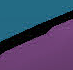
\includegraphics[width=1.0\textwidth]{gibbs}
    \caption{Fenómeno de Gibbs en una imagen JPEG}
    \label{fig:gibbs}
\end{figure}

La imagen ``Klay'' (figura \ref{fig:ref-klay}) es una captura de un pantalla de
un juego cuyo estilo presenta muchos saltos discontinuos.

La imagen ``Diego'' (figura \ref{fig:ref-diego}) es una fotografía que presenta
mucho ruido, gracias al fondo de mármol.

La imagen ``Ghost'' es una captura de pantalla del Anime \emph{Ghost in the
Shell}. Es un punto medio entre el ruído de ``Diego'' y el estilo caricaturesco
de ``Klay''

Finalmente, la imagen ``Pluto'' (figura \ref{fig:ref-pluto}) es una fotografía
publicada por NASA cuando la sonda \emph{New Horizons} pasó cerca de Plutón en
Septiembre de 2015. La imagen tiene una resolución de $8000\times8000$ y su
principal propósito es mostrar cómo se comportan los diferentes componentes del
proyecto cuando se presenta una carga de trabajo grande relativamente a las
demás imágenes.

\begin{figure}[b]
    \includegraphics[width=1.0\textwidth]{ref_klay}
    \caption{Klay}
    \label{fig:ref-klay}
\end{figure}

\begin{figure}[b]
    \includegraphics[width=1.0\textwidth]{ref_diego}
    \caption{Diego}
    \label{fig:ref-diego}
\end{figure}

\begin{figure}[b]
    \includegraphics[width=1.0\textwidth]{ref_ghost}
    \caption{Ghost}
    \label{fig:ref-ghost}
\end{figure}

\begin{figure}[b]
    \includegraphics[width=1.0\textwidth]{ref_pluto}
    \caption{Pluto}
    \label{fig:ref-pluto}
\end{figure}

% ============================================================

% ============================================================
\section{Convergencia}
% ============================================================

Recordando la ecuación que usamos para la función de aptitud:

\begin{equation}
f(T) = \frac{e(T)}{e(T_0)} + \alpha \Big(\frac{s(T)}{s(T_0)}\Big)
\end{equation}\label{eq:fitness-repeated}

Se desea obtener la cota mínima.

Se sabe que $e(T_0)$ es siempre menor o igual a $e(T)$, ya que $T_0$ es la
tabla unitaria, que produce el menor error posible. Por lo tanto, el primer término
de la ecuación está en $[1, \infty)$.

De manera análoga, el tamaño de la imagen resultante al comprimir con la tabla
unitaria es el mayor posible. Entonces, el término $\frac{s(T)}{s(T_0)} \in (0,
1]$. Se encontró que un buen valor de $\alpha$ para conseguir imágenes de alta
calidad es 10. Por lo tanto, el segundo término de la ecuación $f(T)$ está en
el intervalo $(0, 10]$

Esto nos da una cota mínima de 1, pero alcanzar una aptitud de 1 es imposible
ya que requeriría una imagen comprimida de tamaño 0. Para el conjunto de
prueba, los mejores valores de aptitud siempre fueron mayores a 4.

En esta sección se incluyen las gráficas de convergencia para la función de
aptitud al correr gp\_encoder con las cuatro imágenes de referencia:
\ref{img:plot-diego}, \ref{img:plot-ghost}, \ref{img:plot-klay}, \ref{img:plot-pluto}.

Todas las figuras mostradas están normalizadas a 500 generaciones con un rango
de evaluación de la función de aptitud entre 4 y 11. Se usa una gráfica de
línea para mostrar el valor de la función de aptitud para los individuos más
aptos y se utilizan puntos para los peores individuos de cada generación. Se
usan puntos porque comúnmente ocurre que en alguna generación, el individuo
menos apto tenga un valor de aptitud mucho mayor a 11. El caso común, sin
embargo, es que los individuos menos aptos también tienden a un punto de
convergencia mientras la evolución avanza.

\begin{figure}[b]
    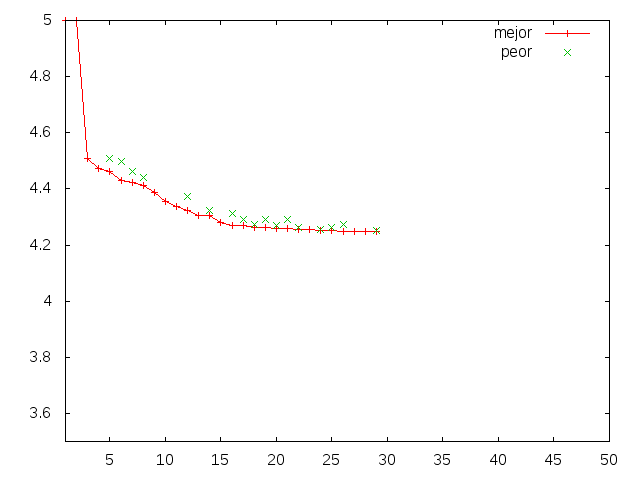
\includegraphics[width=1.0\textwidth]{plot_diego}
    \caption{Convergencia para imagen ``Diego"}
    \label{img:plot-diego}
\end{figure}

\begin{figure}[b]
    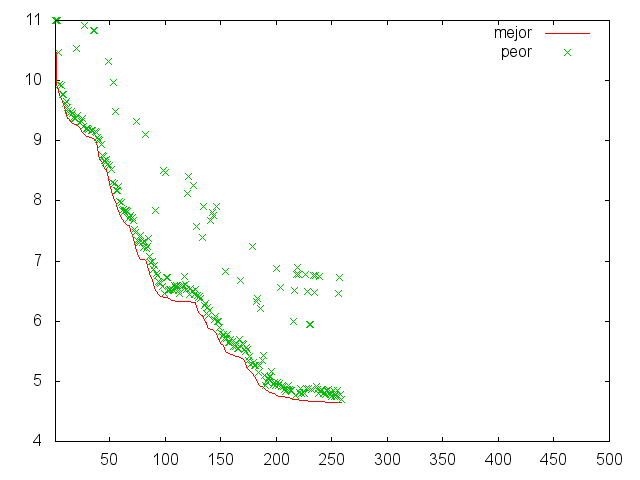
\includegraphics[width=1.0\textwidth]{plot_ghost}
    \caption{Convergencia para imagen ``Ghost"}
    \label{img:plot-ghost}
\end{figure}

\begin{figure}[b]
    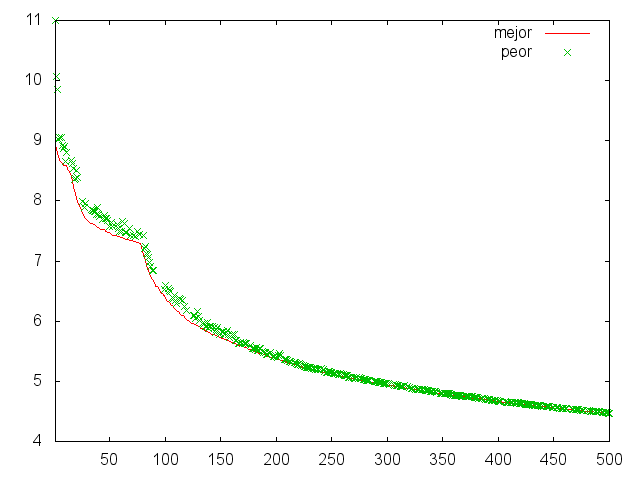
\includegraphics[width=1.0\textwidth]{plot_klay}
    \caption{Convergencia para imagen ``Klay"}
    \label{img:plot-klay}
\end{figure}

\begin{figure}[b]
    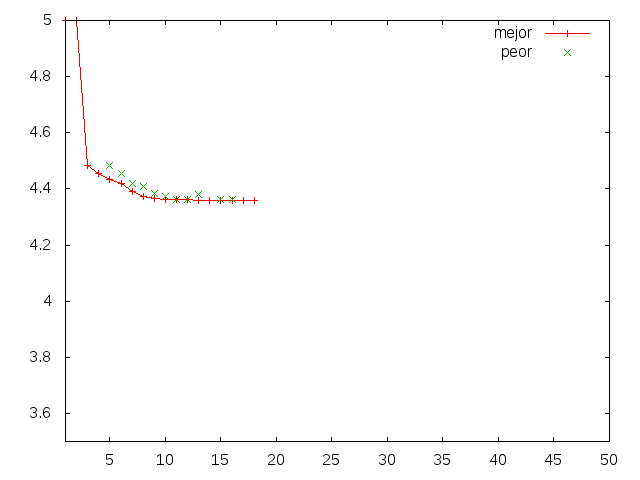
\includegraphics[width=1.0\textwidth]{plot_pluto}
    \caption{Convergencia para imagen ``Pluto"}
    \label{img:plot-pluto}
\end{figure}

% ============================================================
\section{Comparación de resultados}
% ============================================================

La tabla \ref{fig:perf_table} es una copia de la que se mostró en el capítulo
\ref{ch:implementacion}. Muestra el desempeño de gp\_encoder en sus
diferentes modalidades: CPU (single-thread y multi-thread) y GPU (OpenCL).

\begin{figure}[h!]
    \begin{tabular}{ |l c c c c r| }
        \hline
        Nombre &  Un Thread & Múltiples Threads & GPU & Speedup MT & Speedup GPU \\
        \hline
        Diego & 10.796s & 5.210s & 1.391s  & 2.072X & 7.76X \\
        Ghost & 13.706s & 6.607s & 1.760s  & 2.257X & 7.78X \\
        Klay & 40.526s & 22.279s & 4.785s  & 1.819X & 8.46X \\%, 4.65
        Plutón & 558.83s & 204.120s & 13.940s & 2.73X & 40.08X \\ % 14.64
        \hline
    \end{tabular}
    \caption{Tabla de desempeño para gp\_encoder}
    \label{fig:perf_table}
\end{figure}

El algoritmo evolutivo se desarrolló con el propósito de generar imágenes
indistinguibles de las originales pero con una buena tasa de compresión. En la
tabla \ref{fig:size-table} comparamos los tamaños de las imágenes de prueba
originales con su versión comprimida con la tabla de cuantificación
evolucionada y la compresión "media" de TinyJPEG, descrita en el capítulo
\ref{ch:implementacion}.

Con todas las imágenes, gp\_encoder produce en imágenes codificadas de menor
tamaño.

Un problema que por sí solo es un área de investigación \cite{subjective-paper}
es juzgar la calidad percibida de imágenes dada la pérdida de información. Para
este trabajo, se compara la compresión de TinyJPEG a calidad media, que usa la
tabla de cuantificación que se presenta en la especificación de JPEG
multiplicada por la constante $\frac{1}{10}$.

Tanto con TinyJPEG en calidad media como con los resultados de gp\_encoder,
todas las imágenes son indistinguibles de la original, salvo por la imagen
Klay, que se discute adelante. Si ambos codificadores producen imágenes
indistinguibles de la original, entonces el codificador que produzca la imagen más
pequeña es el mejor de los dos.

La imagen Klay, con ambos codificadores, produce defectos al ser comprimida.
Cabe notar que los defectos no fueron distinguibles para un grupo de personas
no familiarizadas con compresión. Para ilustrar la diferencia entre la
imagen Klay comprimida con TinyJPEG y la resultante de gp\_encoder, se incluye
la imagen \ref{img:banding}, con TinyJPEG a la izquierda y gp\_encoder a la
derecha. A la izquierda puede observarse un efecto de bandas de color más
marcado que el que aparece en el lado derecho. La imagen original presenta bandas de
color, sin embargo, la imagen resultante de gp\_encoder no agrega nuevas
bandas, a diferencia de TinyJPEG. Desde este punto de vista, la imagen que
produce gp\_encoder tiene mayor calidad que la de TinyJPEG. Por otro lado, el
Fenómeno de Gibbs es menos notorio en la imagen producida por TinyJPEG.

\begin{figure}
    
\includegraphics[width=400pt, height=200pt]{banding}
    \caption{Izquierda: TinyJPEG. Derecha: gp\_encoder}
    \label{img:banding}
\end{figure}

Para finalizar, se incluye la tabla de cuantificación evolucionada para la
imagen Klay (figura \ref{fig:klay-table}). Vale la pena compararla con la tabla de
cuantificación de referencia \ref{fig:reference-table} para observar las
características poco intuitivas de la tabla generada por gp\_encoder, como la
relativa alta cantidad de coeficientes de valores bajos en las frecuencias
altas.


\begin{equation}
    \begin{matrix}
        1  &   8  &  1  & 20  &  1  & 16  & 38  & 12 \\
        37 &   59 &  44 &  21 &  18 &  14 &   4 &  11 \\
        23 &   54 &  49 &  33 &  42 &  15 &  27 &  45 \\
        53 &   43 &  32 &  34 &   6 &  28 &   6 &   4 \\
        4  &  63  & 39  & 10  & 15  &  2  &  1  &  4 \\
        10 &    1 &  17 &  10 &  28 &   7 &   8 &  47 \\
        46 &   28 &   3 &  20 &   1 &  39 &   8 &  31 \\
        5  &  34  &  4  & 31  & 12  & 15  & 43  & 39
    \end{matrix}
    \label{fig:klay-table}
\end{equation}

\begin{figure}[h]
    \begin{tabular}{|l c c r|}
        \hline
        Nombre & Original & TinyJPEG & gp\_encoder \\
        \hline
        Diego & 2.3M & 355K & 264K \\
        Ghost & 2.6M & 562K & 361K \\
        Klay  & 9.1M & 419K & 221K \\
        Pluto & 192M & 26M  & 19M  \\
        \hline
    \end{tabular}
    \caption{Tamaños de imagen original y con compresión}
    \label{fig:size-table}
\end{figure}


